\section{Backend}

\subsection{Spring}

\subsubsection{Dependency Injection}

Wie bereits erwähnt wurde als Framework für das Java-Backend Spring verwendet. Ein sehr nützliches Design-Konzept von Spring ist die Dependency Injection.

\zitat{Als Dependency Injection wird in der objektorientierten Programmierung ein Entwurfsmuster bezeichnet, welches die Abhängigkeiten eines Objekts zur Laufzeit reglementiert: Benötigt ein Objekt beispielsweise bei seiner Initialisierung ein anderes Objekt, ist diese Abhängigkeit an einem zentralen Ort hinterlegt – es wird also nicht vom initialisierten Objekt selbst erzeugt.}{https://de.wikipedia.org/wiki/Dependency_Injection}

Die Abhängigkeit von einem anderen, existierenden Objekt wird im Code meistens über die \verb|@Autowire| -Annotation gekennzeichnet. Durch Dependency Injection ist es möglich, kurzen, gut leserlichen und gut wartbaren Code zu schreiben. Einerseits weil dadurch sehr viele Dinge nicht implementiert werden müssen, andererseits weil die Komponenten der Applikation klar getrennt werden können, da die Verknüpfungen automatisch zur Laufzeit erstellt werden.

\subsubsection{JavaBeans}
Ein Java Grundkonzept das für das Verständnis von Spring (und bei der Fehlerbehebung während der Applikations- Entwicklung) sehr hilfreich ist, sind JavaBeans. Dabei handelt es sich im Prinzip um ein Entwurfsmuster für Klassendefinitionen. Die entworfene Klasse muss dabei folgenden Ansprüchen genügen:

\begin{itemize}
	\item öffentlicher parameterloser Konstruktor
	\item Serialisierbarkeit (die Klasse ist eine Subklasse von Serializable)
	\item öffentliche Zugriffsmethoden (Public Getters/Setters) die einer Namenskonvention folgen
\end{itemize}

Die Vorteile von JavaBeans lassen sich am besten beschreiben durch:

\zitat{Beans realisieren eine verbesserte Serialisierung und damit Netzwerkfähigkeit, Wiederverwendbarkeit, Portabilität und Interoperabilität.}{https://de.wikipedia.org/wiki/JavaBeans}

Damit stellen JavaBeans ein sehr gutes Konzept für die Durchführung der Dependency Injection dar, weil sie gut erzeug- und verlinkbare Objekte zur Verfügung stellen. In Spring kann die Annotation \verb|@Component| verwendet werden, um eine Klasse als Bean zu kennzeichnen. Im Code werden allerdings die Annotations \verb|@Service|, \verb|@Controller|, und \verb|@Repository| verwendet, die die Klassen als Beans kennzeichnen. Diese drei Annotations sind auf einen bestimmten Zweck hin spezialisierte Ableitungen von \verb|@Component|.

\subsection{Architektur}

\begin{figure}[h]
\centering
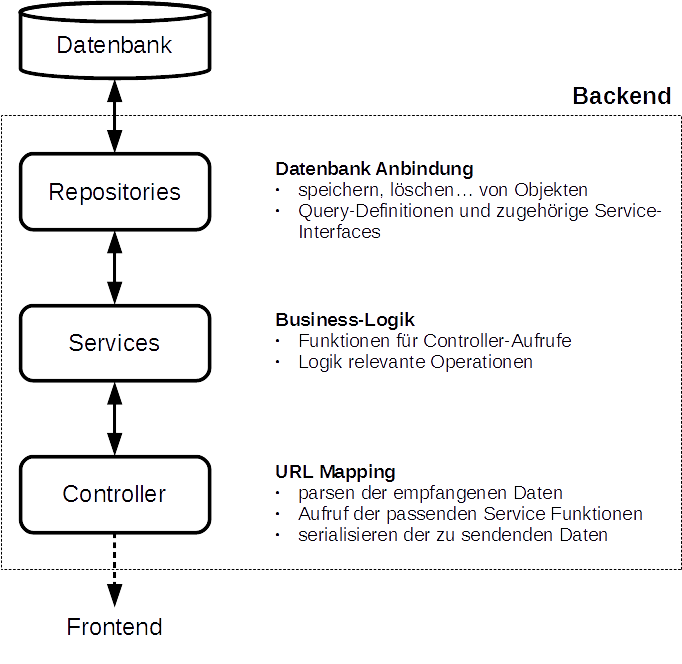
\includegraphics[width=0.8\linewidth]{3_backend/pics/architecture}
\caption{Grobes Architekturdesign des Backends}
\label{fig:architecture_backend}
\end{figure}

In Abbildung \ref{fig:architecture_backend} ist eine grobe Übersicht über die Komponenten des Backends und den zugehörigen Aufgaben zu sehen. Um die Integration neuer Tabellen in das Gesamtschema zu erleichtern wurde für jede Entity-Klasse (jede Tabelle in der Datenbank) eine Klasse von jedem Architektur-Element (\verb|Repository|, \verb|Service|, \verb|Controller|) erstellt. Diese Designentscheidung und die hinter jedem der Architektur-Elemente liegende Logik und Funktion wird in den folgenden Punkten genauer erläutert.

\FloatBarrier
\subsubsection{Entities}\label{sec:entities}

Die Entity-Klassen sind das Zentrum der Backend-Struktur. Da einer der wichtigsten Aspekte des Projekts Anpassbarkeit und Erweiterbarkeit ist, war es wichtig möglichst zentrale, und klar definierte Schnittstellen dafür zu schaffen. Außerdem sollten diese Schnittstellen so unabhängig wie möglich sein, und in wenig Stellen im restlichen Code berücksichtigt werden müssen. Die wesentlichste dieser Schnittstellen ist eine Entity-Klasse. Einerseits wird hier die Verbindung und das Mapping zur Datenbank festgelegt, andererseits sind fast sämtliche Informationen für die De- und Serialisierung in für das Frontend interpretierbare Daten an dieser Stelle festgelegt. In dem Code-Segment \ref{PaymentAccount} ist exemplarisch eine Entity-Klasse abgebildet, anhand der die Funktionalität der einzelnen Komponenten erklärt wird.

\scriptsize
\begin{lstlisting}[caption=PaymentAccount.java, label=PaymentAccount, language=Java]
@Entity
public class PaymentAccount {

	@Id
	@JsonProperty("Depot")
	private String id;
	
	@JsonProperty("Betrag")
	private Integer currentamount;
	
	@OneToMany(mappedBy = "paymentaccount", cascade = CascadeType.ALL)
	@JsonIgnore
	private List<Payment> payments;
	
	public PaymentAccount() {
		this.id = "";
		this.currentamount = 0;
	}
	
	public String getId() { 
		return this.id; 
	}
}
\end{lstlisting}
\normalsize

\nosectionheadline{Verbindung zur Datenbank}

Die im Projekt verwendeten Annotations zur festlegung der JPA-Eigenschaften sind:

\begin{itemize}
	\item \verb|@Entity|: Markiert eine Klasse als Entity Klasse. Für jede Entity-Klasse wird eine neue Tabelle im Datenbankschema angelegt. Alle in der Klasse festgelegten Membervariablen werden auch als Einträge in der Tabelle der Datenbank erstellt. Für jeden Member wird eine Zeile erstellt. Die meisten zur Zeile zugehörigen Attribute wie z.B. der Datentyp werden (sofern möglich) automatisch festgelegt. Für manche Attribute wie z.B. den Zeilen-Namen gibt es aber Wege um sie manuell festzulegen (vgl. z.B. \verb|@Column|).
	\item \verb|@Id|: Kennzeichnet ein Attribut als Primärschlüssel einer Tabelle. Jede Entity-Klasse muss mindestens einen Primärschlüssel festlegen. Es ist aber auch möglich mehrere Attribute als Primärschlüssel festzulegen. Darauf wird später noch näher eingegangen. Beim gezeigten Beispiel wird ein String, der die Bezeichnung des Payment-Accounts enthält als Primärschlüssel verwendet.
	\item \verb|@OneToMany|, \verb|@OneToOne|, \verb|@ManyToOne|...: Damit wird eine Relation zu einer anderen Tabelle festgelegt. Die Bezeichnung der Annotation entspricht dabei der Art der Relation. Diese Annotations werden auf ein Objekt der referenzierten Klasse (= Tabelle) angewandt. Ein Payment-Account kann von mehreren Payments aus referenziert werden (weshalb es sich bei der Membervariable auch um ein \verb|List<>|-Objekt handelt). Der Zusatz \verb|mappedBy| drückt dabei aus, dass es sich bei dieser Seite der Relation nicht um den Owner handelt. Das bedeutet, dass die verweisenden Sekundärschlüssel in der Tabelle des anderen Objekts gespeichert werden. Über \verb|cascade = CascadeType.ALL| wird das Framework angewiesen, Änderungen die sich auf referenzierte Objekte auswirken (in diesem Fall Payments) auch in die Datenbank zu übertragen.
	\item \verb|@EmbeddedId|: Eine (und die im Projekt verwendete) Methode einen zusammengesetzten Primärschlüssel festzulegen.
	\item \verb|@Column|: Explizite Deklaration einer Membervariable als Zeile in einer Tabelle. Mit Hilfe dieser Annotations können auch explizit Namen vergeben werden, auf die ein Member in der Tabelle gemappt wird.
	\item \verb|@Transient|: Kennzeichnet eine Member-Variable die nicht als Zeile in die zugehörige Tabelle übernommen werden soll.
	\item \verb|@GeneratedValue|: Teilt der Datenbank mit, dass die zugehörige Zeile in der Tabelle von der Datenbank selbst automatisch beschrieben wird. Diese Annotation ist für eine automatische Id-Vergabe sehr hilfreich.
\end{itemize}

Die Auswirkungen auf das tatsächliche Datenbankschema können in Abbildung \ref{fig:db_scheme} nachvollzogen werden.

\begin{figure}[h]
	\centering
	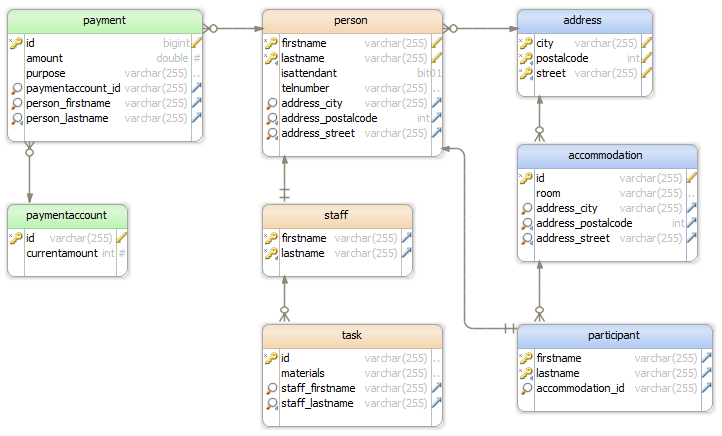
\includegraphics[width=0.9\linewidth]{3_backend/pics/db_scheme}
	\caption{Datenbank Schema}
	\label{fig:db_scheme}
\end{figure}

\nosectionheadline{DeSerialisierung}

Für diese Aufgabe wurde die in Spring bereits integrierte Jackson-JSON-Library verwendet. Diese Library unterstützt das automatische aber gleichzeitig sehr frei definierbare umwandeln von JSON-Objekten auf POJO's (PlainOldJavaObjects). Diese Funktion erweist sich beim Parsen der http-requests sehr nützlich. Dadurch können die empfangenen Daten direkt auf ein POJO gemappt, und das daraus entstehende Objekt ganz normal verwendet werden. Umgekehrt können im Laufe der Backend-Operationen erstellte oder bearbeitete Objekte wieder in für das Frontend verständliche JSON Objekte umgewandelt und zurückgesendet werden. Die verwendeten Annotations werden im folgenden kurz beschrieben:

\begin{itemize}
	\item \verb|@JsonProperty|: Kennzeichnet einen Member explizit als relevant für die Umwandlung in ein JSON-Objekt. Dieser Annotation kann ein Parameter zugeteilt werden, der später in das JSON-Objekt statt dem Member-Namen eingefügt wird. Das erweißt sich vor allem dadurch sehr nützlich, weil im Frontend dann ohne Umwege der Name des Attributes mit dem Wert für die Anzeige verwendet werden kann. Auch werden die Werte von JSON-Objekten, die mit diesem Attribut Namen versehen sind wieder auf diesen Member gemappt.
	\item \verb|@JsonIgnore|: Kennzeichnet eine Member-Variable als nicht relevant für die JSON-DeSerialisierung
	\item \verb|@JsonUnwrapped|: Markiert ein eingebettetes Objekt, das mittels der Library DeSerialisiert werden, und die Membervariablen direkt (also nicht als eigenes Objekt) in das übergeordnete JSON-Objekt integriert werden soll.
	\item \verb|@JsonPropertyOrder|: Definiert die Reihenfolge, mit der die Attribute DeSerialisiert werden sollen.
\end{itemize}

Das POJO \verb|PaymentAccount(id = "Bankkonto", currentamount = 1351.16)| würde \newline dem JSON \verb|{"Depot":"Bankkonto","Betrag":1351.16}| entsprechen.

\nosectionheadline{DeSerialisierung von relationalen Objekten}

Eine Schwierigkeit bei der DeSerialisierung stellten Objekte dar, die über Relationen in die Klasse eingebettet sind. Erstens weil dadurch das Problem der Rekursion entsteht (Objekt A hat eine Membervariable vom Objekt B, das wiederum eine Membervariable vom Objekt C besitzt...). Würde diese Rekursion so umgesetzt werden, müsste ein JSON-Objekt die Informationen des Grundobjekts und aller rekursiv eingebetteten Objekte enthalten. Zweitens ist für die Verwendung eines Objektes meistens nur die Verknüpfung interessant. Es ist wichtig zu wissen, mit welchem(n) Objekt(en) Verknüpfungen bestehen, die Details der verknüpften Objekte werden aber besser an einer anderen Stelle geklärt. Aus diesen Überlegungen heraus, hat sich die Lösung ergeben, die DeSerialisierung solcher Objekte auf die Id's derselben zu reduzieren, da die Id das fremde Objekt eindeutig definiert. Diese Funktionalität wurde mit Hilfe von \verb|@JsonProperty|, das auf Getter und Setter der Foreign-Id angewendet wurde, realisiert. Ein Beispiel hierfür ist im Code-Segment \ref{cs:foreign_id_mapping} zu sehen.

\scriptsize
\begin{lstlisting}[caption=Foreign-Id mapping für die Address-Entity in Person.java, label=cs:foreign_id_mapping, language=Java]
	@EmbeddedId
	@JsonUnwrapped
	private PersonId id;
	
	/* --- content omitted --- */
	
	@JsonProperty("Adresse")
	public AddressId getAddress() {
	   	if(this.address != null)
	   	{
	   		return this.address.getId();
	   	}
	   	else
	   	{
	   		return null;
	   	}
	}
	
	@JsonProperty("Adresse")
	public void setAddressId(String id_string) throws Exception {
	   	if(id_string != null) {
	   		this.address_id = mapper.readValue(id_string, AddressId.class);
	   	}
	   	else {
	   		this.address_id = null;
	   	}
	}
\end{lstlisting}
\normalsize

Ein JSON-Objekt der Person-Entityklasse könnte demnach wie im Code-Segment \ref{cs:person_json}

\scriptsize
\begin{lstlisting}[label = cs:person_json, caption = Beispiel für ein Serialisiertes JSON-Objekt]
{	
	"Nachname":"Pirker",
	"Vorname":"Jakob",
	"Telefonnummer":"123456789",
	"Adresse":{"Strasse":"MeinBlock","Stadt":"MeineStadt","Postleitzahl":1111},
	"Anwesenheit":true
}
\end{lstlisting}
\normalsize

\nosectionheadline{Primärschlüssel mit mehreren Attributen}

Aus der Reduzierung eines Objekts auf seine Id ergibt sich (speziell im Hinblick auf das Frontend) die zusätzliche Anforderung an die Id, dass sie vom User direkt durch Lesen einem Objekt zugeordnet werden können soll. Will man zum Beispiel eine Zahlung einer Person zuordnen, so reichen Vorname und Nachname aus, um die Person eindeutig zu kennzeichnen. Gleichzeitig erfüllt die Kombination der Attribute aber auch die Haupteigenschaft einer Id: Eindeutigkeit. Würde man einer Person zum Beispiel nur eine Zahl als Id zuordnen, wäre diese zwar eindeutig, aber ein User müsste zuerst herausfinden, um welche Person es sich dabei handelt. Diese Anforderung macht Primärschlüssel mit mehreren Attributen notwendig. Dazu gibt es zwei verschiedene Implementierungsmöglichkeiten: \verb|@IdClass| und \verb|@EmbeddedId|. Beide setzen eine Zwischenklasse, die als Id fungiert und von Serializable erbt voraus. 

\begin{itemize}
	\item \verb|@IdClass|
	\begin{itemize}
		\item Vorteile: Id-Klasse muss zwar definiert werden, scheint aber in der Entity-Klasse nicht auf. Dadurch bleibt der Code besser lesbar, weil nur bei der Implementierung darauf geachtet werden muss, dass sich die Id's der Entity-Klasse mit denen der Basisklasse decken. Anschließend braucht nur mehr die Entity-Klasse betrachtet werden.
		\item Nachteile: Doppelter Code, weil für beide Klassen die gleichen Attribute definiert werden müssen. Umständliche DeSerialisierbarkeit.
	\end{itemize}	
	\item \verb|@EmbeddedId|
	\begin{itemize}
		\item Vorteile: Kein doppelter Code. Die Serialisierung erfolgt bei Verwendung der \verb|@JsonUnwrapped| vollkommen automatisch. Bei der Deserialisierung kann der von der Jackson-JSON-Library zur Verfügung gestellte Mapper sehr gut verwendet werden. 
		\item Nachteile: Für eine vollständige Übersicht über die Attribute der Entity-Klasse muss die Id-Klasse explizit mitberücksichtigt werden.
	\end{itemize}
\end{itemize}

Aufgrund der Serialisierbarkeit wurde die \verb|@EmbeddedId|-Variante gewählt. Ein Implementierungsbeispiel ist ebenfalls im Code-Segment \ref{cs:foreign_id_mapping} zu sehen.

\subsubsection{Repositories}
\normalsize
Repositories stellen das Verbindungsglied zur Datenbank dar. Ihre Hauptaufgabe besteht darin, Objekte aus der Datenbank zu löschen bzw. in die Datenbank zu speichern. Außerdem werden in den Repossitories Queries definiert, und Methoden für die Services zur Verfügung gestellt, über die diese auf die Query-Ergebnisse zugreifen können. Die grundlegenden Operationen wie speichern und löschen werden bereits von einer fertigen Basisklasse \verb|CrudRepository<>| zur Verfügung gestellt. Dem Template muss nur noch ein Parameter für den Entity-Typ sowie den Id-Typ gegeben werden. Diese Klasse stellt auch schon einige wichtige Query Methoden zur Verfügung (Objekte Anhand der Id auslesen, alle Objekte auslesen...). Es ist in Spring nicht notwendig, die Repository-Interfaces explizit in eigenen Klassen zu implementieren. Spring stellt aus einer Interface Definition für ein Repository automatisch die dazugehörige Implementierung her. 

Ein sehr praktisches Feature dabei sind die sogenannten Named-Queries. Folgt der Methoden-Name in einem Repository-Interface einer bestimmten Form, so kann Spring aus dem Namen die zugehörige SQL-Query selbst bestimmen. Somit kann Query- und Methoden-Definition in einem Zug erledigt werden, was die Wartbarkeit, Lesbarkeit und Änderbarkeit des Codes sehr verbessert. Der Methodenname setzt sich dabei aus den Membernamen der zugehörigen Entity-Klasse und aus Keywords zusammen, die es ermöglichen die Member logisch zu verknüpfen. Ein Beispiel für eine mögliche Named-Query im \verb|PersonRepository| wäre:

\scriptsize
\begin{lstlisting}[language=Java]
	List<Person> findByLastnameAndIsattendantOrderByLastnameAsc(String lastname, Boolean isattendant);
\end{lstlisting}
\normalsize
Mit dieser Query würde man aus der Person-Tabelle die Personen mit den in den Funktionsparametern gegebenen Werten für  \verb|lastname| und  \verb|isattendant| herausfiltern, und sie aufsteigend nach dem Nachnamen sortiert bekommen.

Weil oft für alle oder mehrere Objekte die gleichen Queries definiert werden sollen wurde ein Basis-Interface erstellt, das diese gemeinsamen Methoden enthält. Die Implementierung ist in Code-Segment \ref{cs:AbstractRepository} zu sehen. Das Interface ist von \verb|CrudRepository<>| abgeleitet, wodurch die endgültigen Repositories nur mehr von \verb|AbstractRepository<>| abgeleitet werden müssen. Außerdem ist \verb|AbstractRepository<>| mit der Annotation \verb|@NoRepositoryBean| versehen. Dadurch wird für dieses Interface keine eigene Klasse erzeugt, was auch gar nicht möglich wäre, da es sich um ein Template handelt. Die abgeleiteten Repositories können natürlich wieder eigene Named-Queries definieren, bieten aber auch gleichzeitig die Methoden von \verb|AbstractRepository<>| an. Die Implementierung eines abgeleiteten Interfaces ist in Code-Segment \ref{cs:PersonRepository} zu sehen.

\scriptsize
\begin{lstlisting}[caption=AbstractRepository.java, label=cs:AbstractRepository, language=Java]
@NoRepositoryBean
public interface AbstractRepository<T_obj, T_id extends Serializable> extends CrudRepository<T_obj, T_id> {
	Iterable<T_obj> findAllByOrderByIdAsc();
}
\end{lstlisting}

\begin{lstlisting}[caption=PersonRepository.java, label=cs:PersonRepository, language=Java]
public interface PersonRepository extends AbstractRepository<Person, PersonId> {
}
\end{lstlisting}
\normalsize

\subsubsection{Controller}

Wie bereits erwähnt existiert für jede Entity-Klasse u.A. auch eine Controller-Klasse. Sie stellt die Schnittstelle zum Frontend dar, indem URL-Aufrufe auf bestimmte Funktionsaufrufe gemappt werden. Jede Entity-Klasse soll im Endeffekt über das Frontend bearbeitbar sein. Für jedes Objekt soll es dabei einen Grundsatz an Funktionen geben, der für jede Entity verfügbar ist. In der \verb|AbstractController<>|-Klasse (vgl. Code-Segment \ref{cs:AbstractController}) wird genau dieser Grundsatz definiert. Dabei werden folgende Requests folgenden Responses zugeordnet:

\begin{itemize}
	\item \textbf{GET-Request}  auf Basis-URL: String, der die Struktur der Entity beschreibt. Dieser Teil wird im Rahmen der Services noch genauer beschrieben.
	\item \textbf{POST-Request}  auf Basis-URL: Speichern eines neuen Objekts in die Datenbank. Das neue, zu speichernde Objekt wird dabei über \verb|@RequestBody| aus den Daten des http-Requests extrahiert. Die Daten werden Dabei in Form eines JSON-Objektes erwartet, \verb|@RequestBody| mappt dieses JSON-Objekt direkt auf das in der Argumentliste definierte POJO. Als Antwort auf diesen Request wird das gespeicherte Objekt gesendet. Dieses wird implizit über die Jackson-JSON-Library in ein JSON-Objekt umgewandelt, das in die Daten der http-Response geschrieben wird.
	\item \textbf{DELETE-Request}  auf Basis-URL: Löschen eines Objektes aus der Datenbank. Das zu löschende Objekt wird gleich wie beim POST-Request aus den Request-Daten extrahiert.
	\item \textbf{GET-Request}  auf Basis-URL+ '/list': Liste von allen Objekten des vorgegebenen Typs in der Datenbank. Auch hier wird die erzeugte Liste wie beim POST-Request implizit in ein JSON-Objekt serialisiert, und in den Daten der http-Response gesendet.
\end{itemize}

Für einen konkreten Controller muss dann nur (wie in Code-Segment \ref{cs:PersonController} zu sehen) eine Klasse erstellt werden, die von dieser Basisklasse erbt. Wichtig ist hier auch noch, über \verb|@RequestMapping|  den URL-Pfad, über den die Entität verfügbar ist zu mappen. Auch wichtig ist hier, dass die Klasse mit \verb|@RestController| gekennzeichnet wird. Damit wird wie schon beschrieben eine JavaBean erzeugt, die u.A. mittels \verb|@Autowired| automatisch zugewiesen werden kann. Bei der abstrakten \verb|AbstractController<>| Klasse muss diese Annotaion natürlich weggelassen werden, da es sich a) um eine abstrakte Klasse und b) um ein Template handelt.

\scriptsize
\begin{lstlisting}[caption=AbstractController.java, label=cs:AbstractController, language=Java]
public abstract class AbstractController<T_obj extends Object, T_serv extends AbstractServiceInterface<T_obj>> {

	@Autowired
	protected T_serv service_;
	
	@RequestMapping(method = RequestMethod.GET)
	public String getRequest() {
		return service_.getJsonStringWithForeignIds();
	}
	
	@RequestMapping(method = RequestMethod.POST)
	public T_obj postRequest(@RequestBody T_obj new_obj) {
		return this.service_.save(new_obj);
	}
	
	@RequestMapping(method = RequestMethod.DELETE)
	public void deleteRequest(@RequestBody T_obj delete_obj) {
		this.service_.delete(delete_obj);
	}
	
	@RequestMapping(value = "/list", method = RequestMethod.GET)
	public Iterable<T_obj> getList() {
		return service_.getList();
	}
}
\end{lstlisting}

\begin{lstlisting}[caption=PersonController.java, label=cs:PersonController, language=Java]
@RestController
@RequestMapping("/person")
public class PersonController extends AbstractController<Person, PersonService>{
}
\end{lstlisting}
\normalsize

Ein GET-Request auf die URL \verb|http://localhost:8080/person/list| könnte folgende Response-Daten liefern:

\scriptsize
\begin{lstlisting}
[
	{	
	"Nachname":"Pirker",
	"Vorname":"Jakob",
	"Telefonnummer":"123456789",
	"Adresse":{"Strasse":"MeinBlock","Stadt":"MeineStadt","Postleitzahl":1111},
	"Anwesenheit":true
	},
	{	
	"Nachname":"Mustermann",
	"Vorname":"Max",
	"Telefonnummer":"987654321",
	"Adresse":{"Strasse":"AuchMeinBlock","Stadt":"AuchMeineStadt","Postleitzahl":2222},
	"Anwesenheit":false
	}
]
\end{lstlisting}
\normalsize

\subsubsection{Services}
Der Service Stellt im Prinzip die Verbindung zwischen Repositories und Controllern her. Natürlich können hier auch Anwendungsspezifische Erweiterungen in der Logik implementiert werden. Um die grundsätzliche Funktionalität möglichst einfach zu gewährleisten wurde auch hier eine abstrakte Template - Klasse erzeugt, die die Standardoperationen nativ unterstützt (s. Code-Segment \ref{cs:AbstractService}).

\scriptsize
\begin{lstlisting}[caption=AbstractService.java, label=cs:AbstractService, language=Java]
public abstract class AbstractService<T_obj, T_id extends Serializable, T_rep extends AbstractRepository<T_obj, T_id>> implements AbstractServiceInterface<T_obj>{

	@Autowired
	protected T_rep base_repository_;
	
	protected ObjectMapper object_mapper_ = new ObjectMapper();
	
	public T_obj save(T_obj save_object){
		return this.base_repository_.save(save_object);
	}
	
	public void delete(T_obj delete_obj) { 
		this.base_repository_.delete(delete_obj);
	}
	
	public Iterable<T_obj> getList(){
		return base_repository_.findAllByOrderByIdAsc();
	}
}
\end{lstlisting}
\normalsize

Grundsätzlich kann diese Basisklasse wie auch schon beim Controller direkt verwendet werden. Ein wesentlicher Punkt, den sie aber nicht automatisiert beherrscht ist der Umgang mit Fremdschlüsseln. Dieser muss für jede Entität die Fremdschlüssel enthält eigens festgelegt werden. Ein Beispiel hierfür ist in Code-Segment \ref{cs:PersonService} anhand des PersonServices zu sehen.

\scriptsize
\begin{lstlisting}[caption=PersonService.java, label=cs:PersonService, language=Java]
@Service
public class PersonService extends AbstractService<Person, PersonId, PersonRepository>{

	@Autowired
	private AddressRepository address_repository_;
	
	@Override
	public Person save(Person save_person){
	
		// try to insert the valid address-object from the DB by it's id (from JSON)
		if(save_person.getAddress() == null && save_person.getAddressId() != null)
		{
			save_person.setAddress(address_repository_.findOne(save_person.getAddressId()));
		}
			return this.base_repository_.save(save_person);
		}
	
	public String getJsonStringWithForeignIds() {
	
		JsonNode person = object_mapper_.valueToTree(new Person());
		JsonNode address_ids = object_mapper_.createArrayNode();
		
		Iterable<Address> addresses = address_repository_.findAll();
		
		for(Iterator<Address> i = addresses.iterator(); i.hasNext(); ) {
			((ArrayNode) address_ids).add(object_mapper_.valueToTree(i.next().getId()));
		}
		
		((ObjectNode) person).put("Adresse", address_ids);
		
		return person.toString();
	}
}
\end{lstlisting}
\normalsize

Beim Speichern müssen die Fremdschlüssel berücksichtigt werden. Da Objekte bei der Serialisierung wie in Abschnitt \ref{sec:entities} bereits erläutert, nur die Id hinterlegt wird, muss (wie in \verb|save()| zu sehen) beim speichern das betreffende Objekt noch richtig gesetzt werden (die Speicherung folgt dann über die auch in \ref{sec:entities} beschriebene Kaskadierung automatisch).

Auch bei der Beschreibung der Entity-Struktur müssen die Fremdschlüssel berücksichtigt werden. Einerseits muss dem Frontend irgendwie bekannt gemacht werden, dass es sich bei diesem Objekt um den zugehörigen Fremdschlüssel handelt, andererseits wäre es sehr wünschenswert, wenn die verfügbaren Fremdschlüssel bei der Erstellung eines neuen Entity-Objekts gleich verfügbar wären, um eine leichte Auswahl zu ermöglichen. Das wird genau in der Methode  \verb|getJsonStringWithForeignIds()| realisiert. Es wird einfach ein neues Objekt vom geforderten Typ erzeugt, und in ein JSON-Objekt umgewandelt. Die verfügbaren Fremdschlüssel werden dann nachträglich als Liste (wieder als JSON-Objekte) in das leere Objekt, statt dem leeren Verweis auf einen Fremdschlüssel eingefügt. 
